% !TeX root = main.tex
\chapter{Additional Figures}
\label{appendix:additional_figures}

This appendix collects supporting diagnostic figures that are useful for interpreting Chapter~\ref{chap:evaluation}, but too detailed for the main evaluation flow.

\section{FedAsync Accepted-Update Staleness}
\label{appendix:fedasync_staleness_heatmap}

Figure~\ref{fig:appendix_network_fedasync_participation_staleness} gives the \texttt{FedAsync}-only accepted-update trace corresponding to the buffered asynchronous diagnostics in Section~\ref{sec:eval_network_heterogeneity}. Because \texttt{FedAsync} applies one reply at a time, its server step is also a completed client trip.

\begin{figure}[H]
\centering
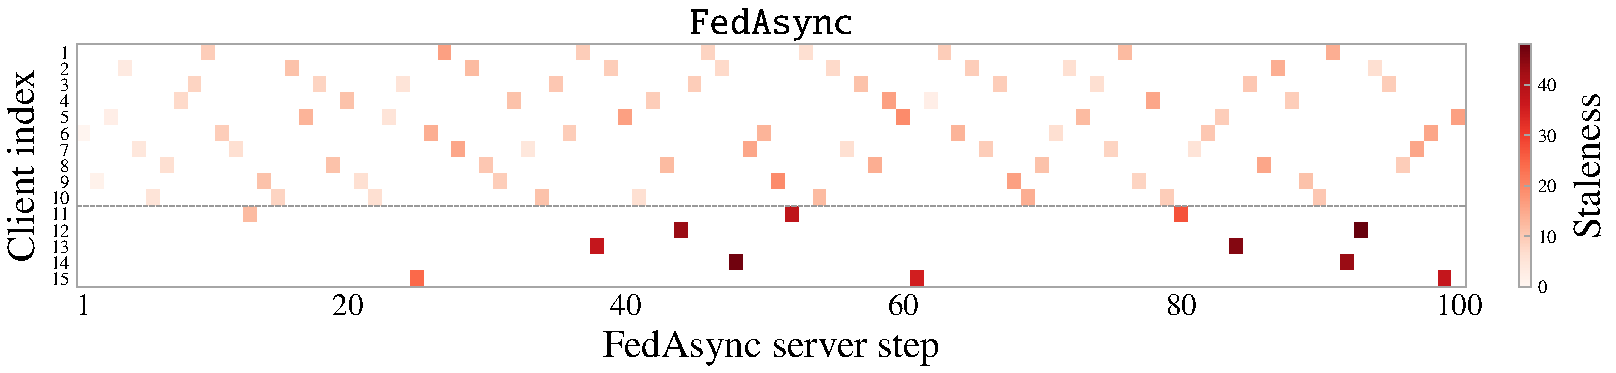
\includegraphics[width=\textwidth]{figures/network_fedasync_participation_staleness.pdf}
% Notes: rows 1--10 are rpi5 client slots; rows 11--15 are rpi4 client slots.
% White cells indicate no accepted update; darker blue indicates larger accepted-update staleness.
\caption{\textbf{\texttt{FedAsync} accepted client updates in mixed non-IID runs.} The heatmap shows the first \(100\) accepted updates on the mixed \texttt{rpi5}/\texttt{rpi4} topology, using the same device-slot convention as Figure~\ref{fig:network_async_participation_staleness}.}
\label{fig:appendix_network_fedasync_participation_staleness}
\end{figure}

\section{Fashion-MNIST Local Submodel Accuracy}
\label{appendix:fashion_mnist_local_submodel_dist}

Figure~\ref{fig:appendix_compute_fashion_mnist_local_submodel_grid} gives the Fashion-MNIST counterpart to the CIFAR-10 local-submodel diagnostic in Figure~\ref{fig:compute_cifar10_seed1340_local_submodel_grid}. It pools the per-client extracted-submodel evaluations from seeds \texttt{1337}, \texttt{1338}, and \texttt{1339}.

\begin{figure}[H]
\centering
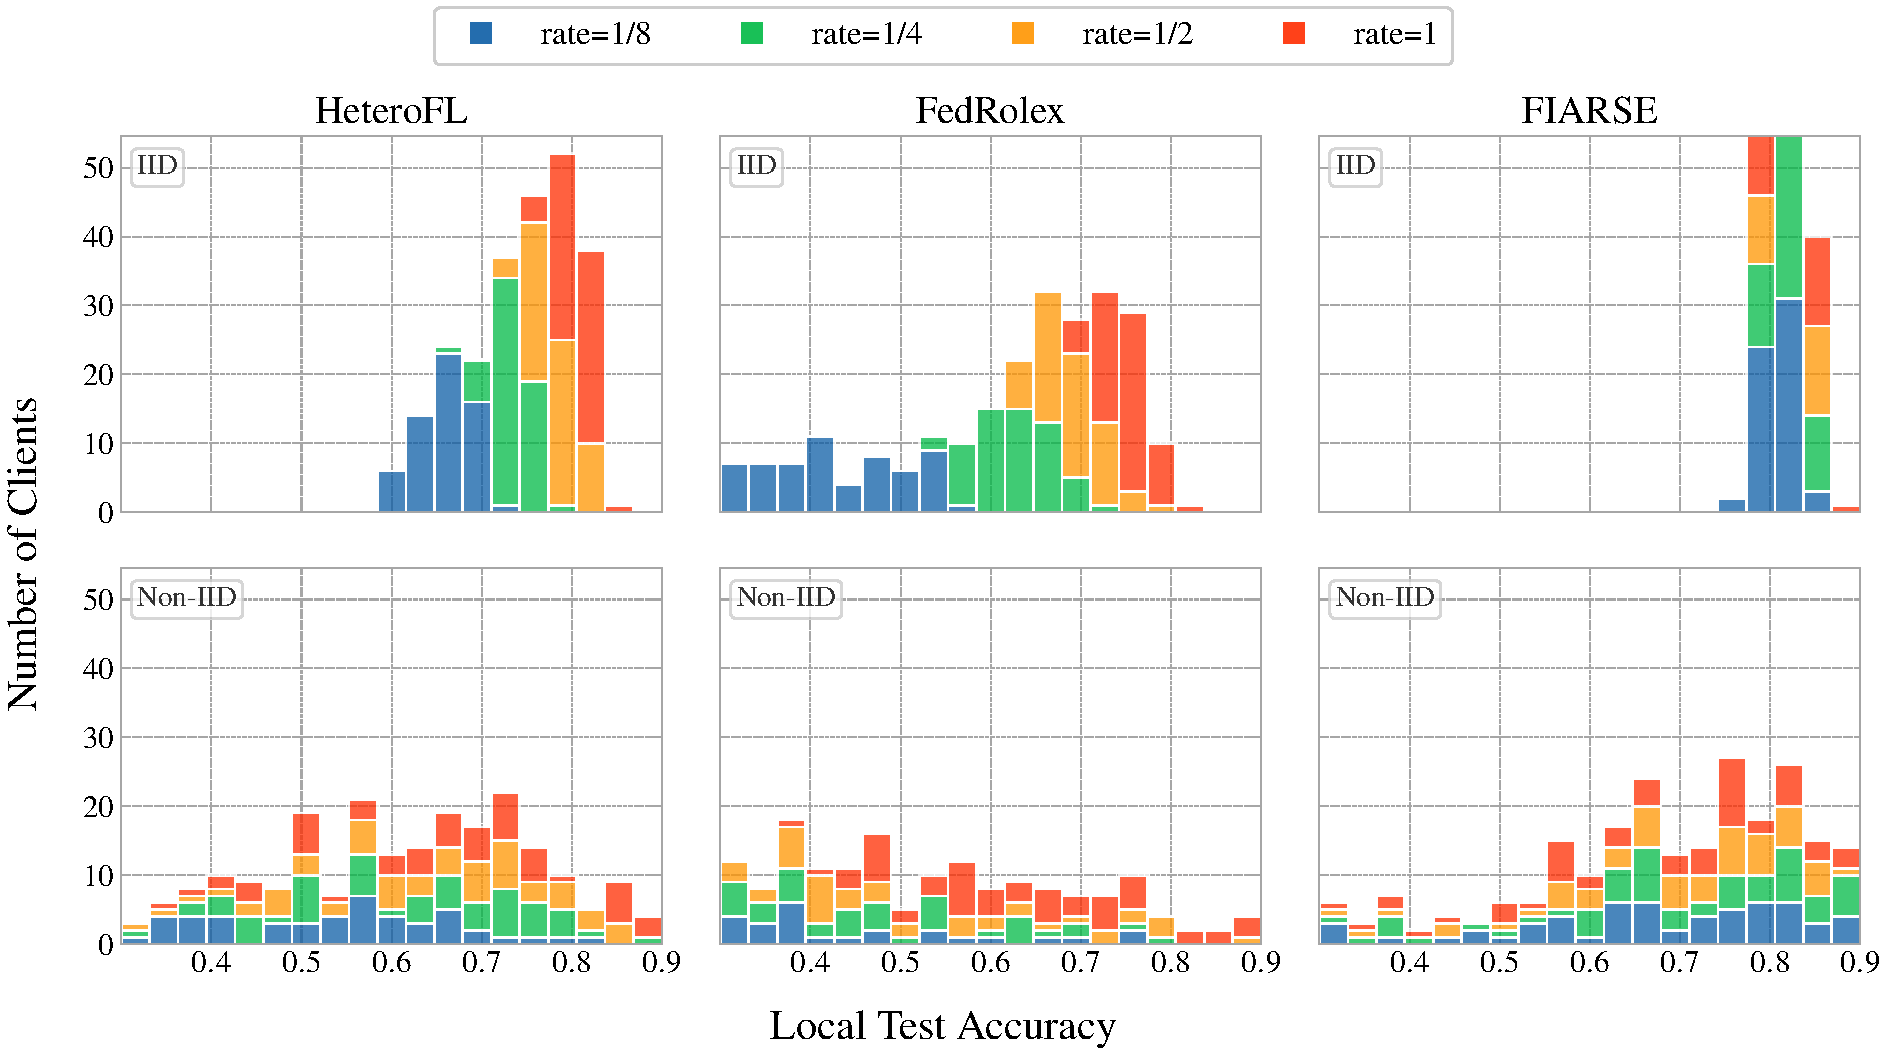
\includegraphics[width=0.98\textwidth]{figures/compute_main_fashion_mnist_local_submodel_grid.pdf}
% Notes: rows are IID/non-IID and columns are HeteroFL, FedRolex, and FIARSE.
% Each panel pools final local-submodel evaluations for rates 0.125, 0.25, 0.5, and 1.0 across seeds 1337, 1338, and 1339.
% Accuracy is measured on each client's local evaluation partition, not the global test set.
\caption{\textbf{Client-level Fashion-MNIST local submodel accuracy distributions.}}
\label{fig:appendix_compute_fashion_mnist_local_submodel_grid}
\end{figure}

\section{Fashion-MNIST Client Training Time}
\label{appendix:fashion_mnist_client_train_time}

Figure~\ref{fig:appendix_compute_fashion_mnist_client_train_time} gives the Fashion-MNIST counterpart to the CIFAR-10 timing diagnostic in Figure~\ref{fig:compute_cifar10_client_train_time}. It uses seed \texttt{1338} and the same device-rate grouping convention.

\begin{figure}[H]
\centering

\includegraphics[width=0.98\textwidth]{figures/compute_main_fashion_mnist_seed1338_client_train_time.pdf}
% Notes: rows are IID/non-IID and columns are HeteroFL, FedRolex, and FIARSE.
% Curves show mean update_train_duration_s for each device/rate group per server round.
% Shaded bands show within-group standard deviation across clients.
% IID runs contain 20 rounds; non-IID runs contain 40 rounds.
\caption{\textbf{Per-round client training time on Fashion-MNIST.}}
\label{fig:appendix_compute_fashion_mnist_client_train_time}
\end{figure}
